\chapter{The Dot Product}
% Reference for diagrams:https://www.mathsisfun.com/algebra/vectors-dot-product.html

If you have two vectors $u = [u_1, u_2, \dots, w_n]$ and $v = [v_1, v_2,\dots, v_n]$ , 
we define the \newterm{dot product} $u \cdot v$ as 
\begin{equation*}
     u \cdot v = (u_1 \times v_1) + (u_2 \times v_2) + \dots + (u_n \times v_n)
\end{equation*} 

For example, 
\begin{equation*}
    [2,4, -3] \cdot [5, -1, 1] = 2 \times 5 + 4 \times -1 + -3 \times 1 = 3
\end{equation*}\index{dot product}

This may not seem like a very powerful idea, but dot products are \emph{incredibly} useful. 
The enormous GPUs (Graphics Processing Units) that let video games render scenes so quickly? 
They primarily function by computing huge numbers of dot products at mind-boggling speeds. 

\begin{Exercise}[title={Basic dot products}, label=dot_products]
    Compute the dot product of each pair of vectors:
    \begin{itemize}
        \item $[1, 2, 3]$, $[4, 5, -6]$
        \item $[\pi, 2\pi]$, $[2, -1]$
        \item $[0,0,0,0]$, $[10,10,10,10]$
    \end{itemize}
\end{Exercise}
\begin{Answer}[ref=dot_products]
        \begin{itemize}
            \item $[1, 2, 3] \cdot [4, 5, -6] = 4 + 10 - 18 = -4$
            \item $[\pi, 2\pi] \cdot [2, -1] = 2\pi - 2\pi = 0$
            \item $[0,0,0,0] \cdot [10,10,10,10] = 0 + 0 + 0 + 0 = 0$ 
        \end{itemize}
\end{Answer}

\section{Properties of the dot product}

Sometimes we need an easy way to say ``The vector of appropriate length is filled with zeros.''
We use the notation $\vec{0}$ to represent this. Then, for any vector $v$, this is true:

$$v \cdot \vec{0} = 0$$

The dot product is commutative:

$$v \cdot u = u \cdot v$$

The dot product of a vector with itself is its magnitude squared:

$$ v \cdot v = |v|^2 $$

If you have a scalar $a$, then:

    $$(v) \cdot (a u) = a (v \cdot u)$$

So, if $v$ and $w$ are vectors that go in the same direction,

    $$v \cdot w = |v| |w|$$

If $v$ and $w$ are vectors that go in opposite directions,

    $$v \cdot w = -|v| |w|$$
    
if $v$ and $w$ are vectors that are perpendicular to each other, their dot product is zero:

  $$ v \cdot w = 0 $$

\section{Cosines and dot products}

Furthermore, dot products' interaction with cosine makes them even more useful is what makes them so useful: 
If you have two vectors $v$ and $u$,

$$v \cdot u = |v| |u| \cos \theta$$

where $\theta$ is the angle between them.

So, for example, if two vectors $v$ and $u$ are perpendicular, the angle between them is $\pi/2$.  
The cosine of $\pi/2$ is 0. The dot product of any two perpendicular vectors is always 0. In fact, if 
the dot product of two non-zero vectors is 0, the vectors \textit{must be} perpendicular.
% diagram needed 

\begin{Exercise}[title={Using dot products}, label=cos_dot_products]
    What is the angle between these each pair of vectors:
    \begin{itemize}
        \item $[1, 0]$, $[0, 1]$
        \item $[3,4]$, $[4,3]$
    \end{itemize}
\end{Exercise}
\begin{Answer}[ref=cos_dot_products]
        \begin{itemize}
            \item $[1,0] \cdot [0,1] = 0$.  The angle must be $\pi/2$.
            \item $[3,4] \cdot [4, 3] = 24$. $|[3,4]| |[4,3]| \cos(\theta) = 24$. 
            $\cos(\theta) = \frac{24}{(5)(5)}$. $\theta = \arccos(\frac{24}{25}) \approx 0.284 \text{ radians}$.
        \end{itemize}
\end{Answer}

If you have two non-zero vectors $v$ and $u$, you can always compute the angle between them:\index{vectors!angle between}

$$\theta = \arccos(\frac{v \cdot u}{|v| |u|})$$
% Breif Description of arccos
\section{Dot products in Python}

NumPy will let you do dot products using the the symbol @.  Open \filename{first\_vectors.py} 
and add the following to the end of the script:

\begin{Verbatim}
    # Take the dot product
    d = v @ u
    print("v @ u =", d)
    
    # Get the angle between the vectors
    a = np.arccos(d / (mv * mu))
    print(f"The angle between u and v is {a * 180 / np.pi:.2f} degrees")    
\end{Verbatim}

When you run it you should get:
\begin{Verbatim}
v @ u = 4
The angle between u and v is 78.55 degrees
\end{Verbatim}

\section{Work and Power}
%diagram here
Earlier, we mentioned that mechanical work is the product of the 
force you apply to something and the amount it moves. For example, if you 
push a train with a force of 10 newtons as it moves 5 meters, you have done 50 joules of work.

What if you try to push the train sideways? It moves down the track 5 meters, 
but you push it as if you were trying to derail it --- perpendicular to its motion.  
You have done no work, because the train didn't move at all in the direction you were pushing.

% 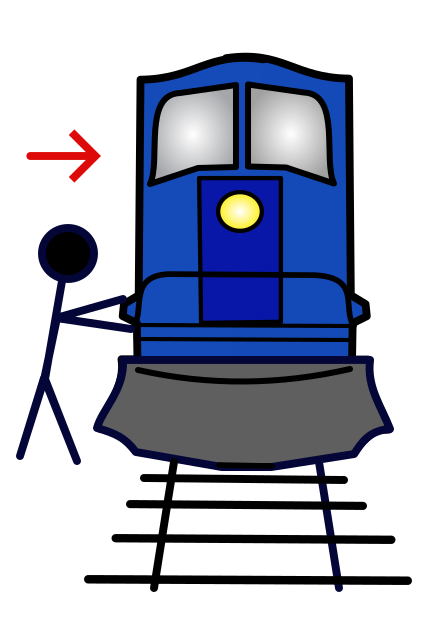
\includegraphics[width=0.8\textwidth]{train.png}


Now that you know about dot products: The work you do is the dot
product of the force vector you apply and the displacement vector of the train. (The displacement
vector is the vector that tells how the train moved while you pushed it.) \index{work}

Similarly, we mentioned that power is the product of the force you apply and the velocity of the
mass you are applying it to. It is actually the dot product of the force vector and the velocity vector.\index{power}

For example, if you are pushing a sled with a force of 10 newtons and it is moving 2 meters per second, 
but your push is 20 degrees off, you aren't transferring 20 watts of power to the sled.  
You are transferring $10 \times 2 \times \cos(20 \text{ degrees}) \approx 18.8$ watts of power.
%add ramps and sin

